\section{Population sizes}

Figure \ref{fig:r_squared_pop} show the same data as was shown in Figure \ref{fig:r_squared} with the population sizes plotted as well. For long polymers the population fluctuates significantly and this is most likely influences the found values for $\langle r^2 \rangle$.
\begin{Figure}
  \centerfloat
     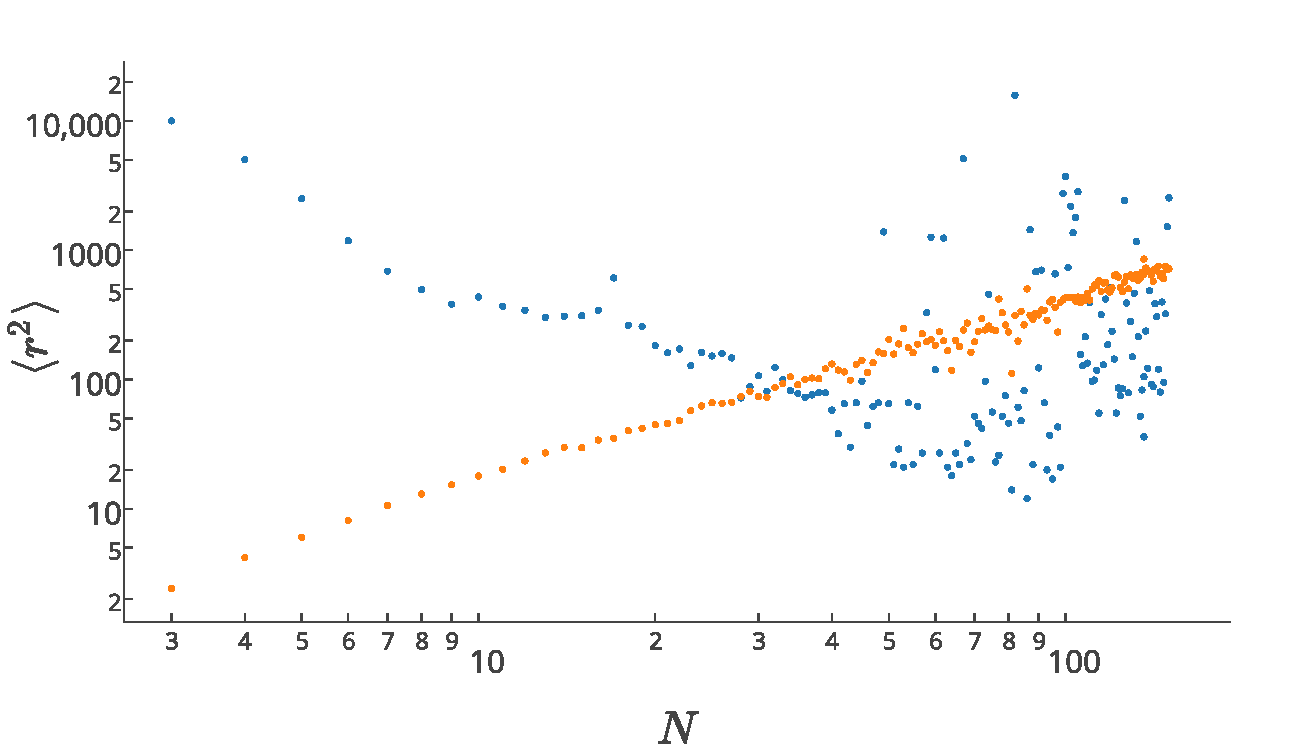
\includegraphics[width=\linewidth]{r_squared_pop.pdf}
 \captionof{figure}{End to end distance $\langle r^2 \rangle$ as function of polymer length $N_l$, with corresponding population sizes.}\label{fig:r_squared_pop}
\end{Figure}

\section{Bending energy}

\begin{Figure}
  \centerfloat
     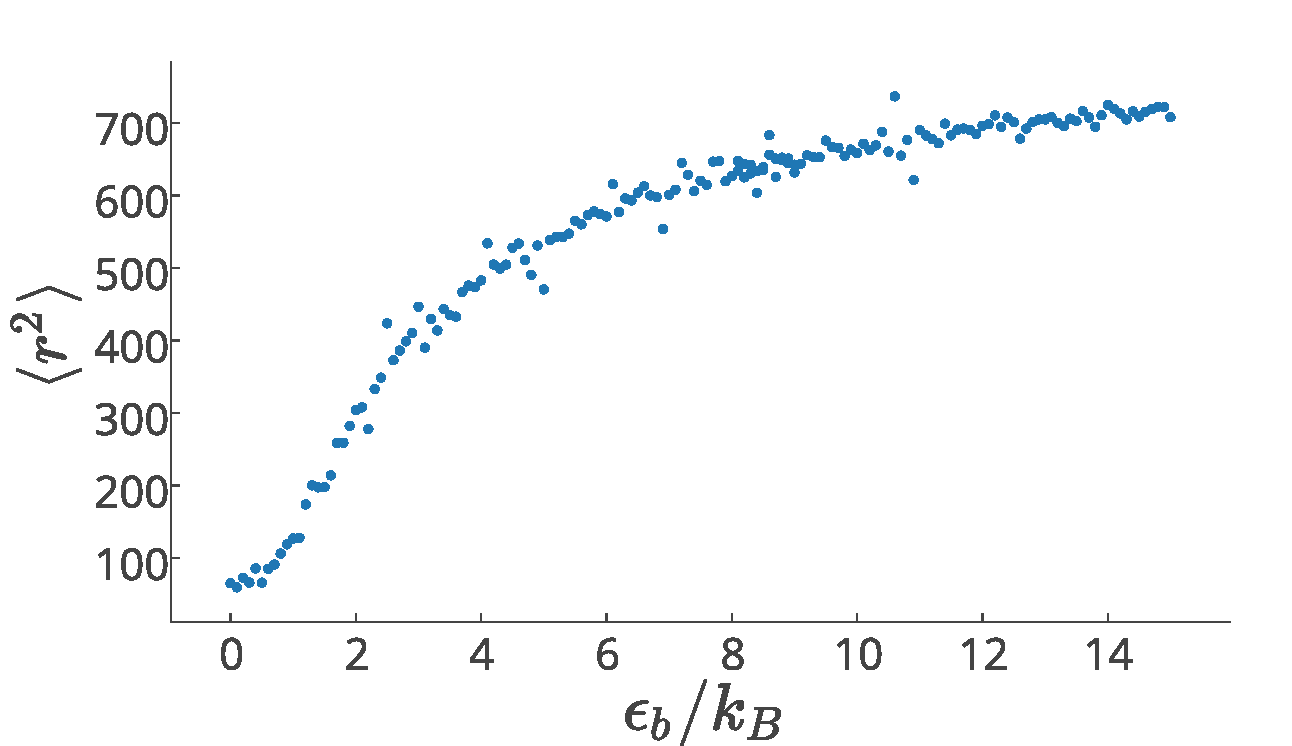
\includegraphics[width=\linewidth]{r_squared_bending.pdf}
 \captionof{figure}{}\label{fig:r_squared_bending}
\end{Figure}